\section{Related work}

\subsection{Multi-objective path planning}

\begin{frame}{Graph based approach}{Multi-objective path planning}
\begin{itemize}
\item Discretization $ \rightarrow $ graph topology
\item Vector-based cost
\item Multi-objective A$ ^{*}$
\end{itemize}
Drawbacks
\begin{itemize}
\item information lose
\item discretization resolution
\end{itemize}
\end{frame}

\begin{frame}{Point-equivalence based approach}{Multi-objective path planning}
\begin{itemize}
\item Direction or waypoint 
\item Encode into solution
\item Evolutionary algorithm
\end{itemize}
Drawbacks
\begin{itemize}
\item obstacles $ \rightarrow $ discontinuity
\item giant search space
\end{itemize}
\end{frame}

\subsection{MOEA-D}

\begin{frame}{Decomposition method}{MOEA-D}
	Decompose a multi-objective optimization problem into subproblems
	\begin{itemize}
		\item Weighted sum approach
		\item Tchebycheff approach
		\item Boundary intersection approach
	\end{itemize}
\end{frame}

\begin{frame}{Weighted sum approach}{MOEA-D}
	\begin{figure}
		\centering
		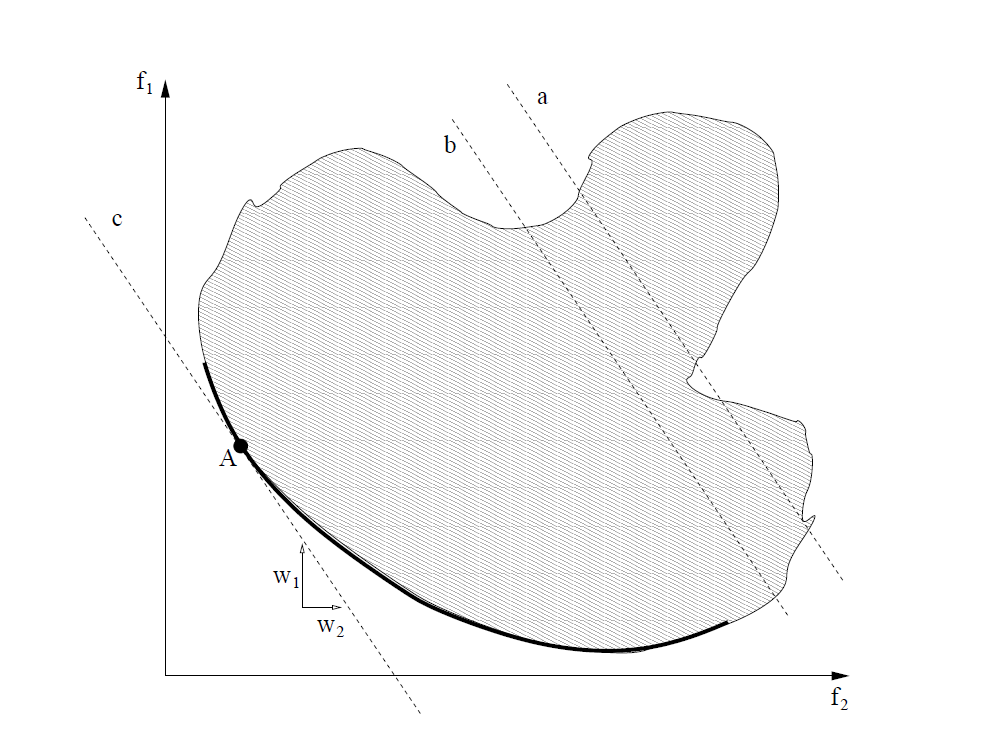
\includegraphics[width=.6\linewidth]{figure/weighted_sum}
		%\caption{}
		\label{fig:weighted_sum}
	\end{figure}
\end{frame}

\begin{frame}{Tchebycheff approach}{MOEA-D}
	\begin{figure}
		\centering
		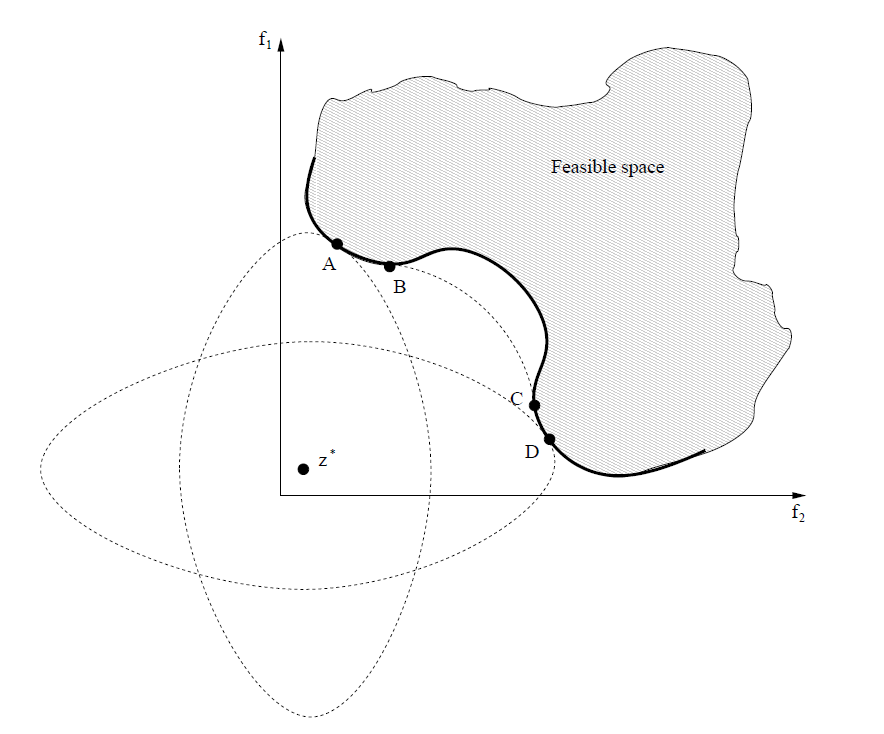
\includegraphics[width=.6\linewidth]{figure/tchebycheff}
		%\caption{}
		\label{fig:tchebycheff}
	\end{figure}	
\end{frame}

\begin{frame}{Boundary intersection approach}{MOEA-D}
	\begin{figure}
		\centering
		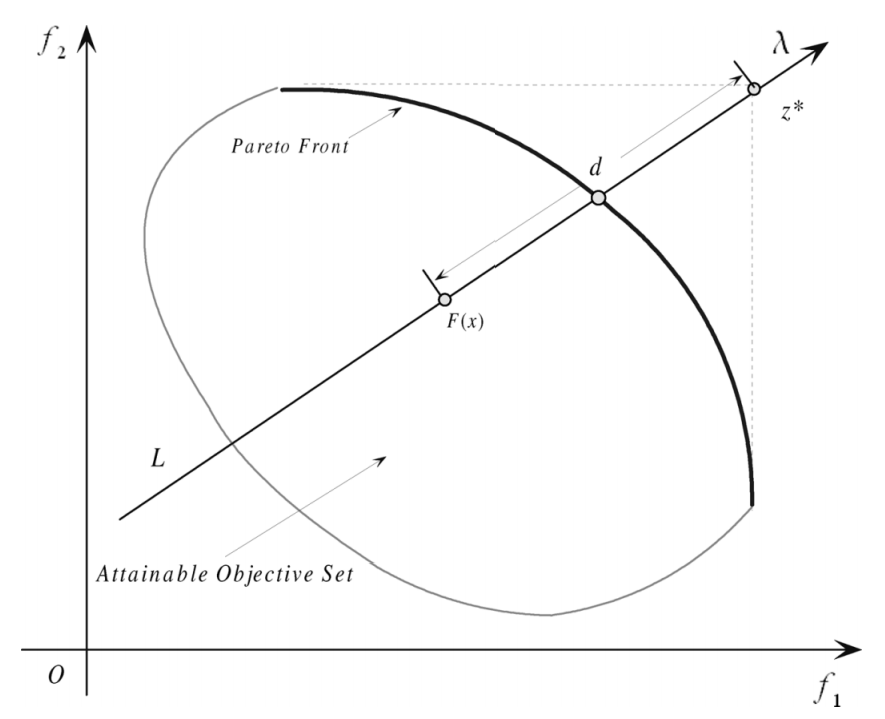
\includegraphics[width=.6\linewidth]{figure/boundary_intersection}
		%\caption{}
		\label{fig:boundary_intersection}
	\end{figure}	
\end{frame}

\subsection{RRT$^{*}$}

\begin{frame}{RRT}{RRT$^{*}$}
	\begin{figure}
		\centering
		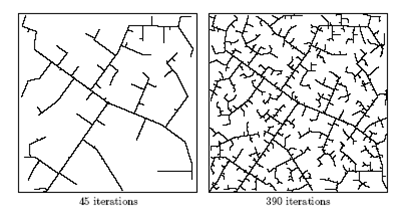
\includegraphics[width=.5\linewidth]{figure/RRT_graph1}
		%\caption{}
		\label{fig:rrt}
	\end{figure}
	\begin{figure}
		\centering
		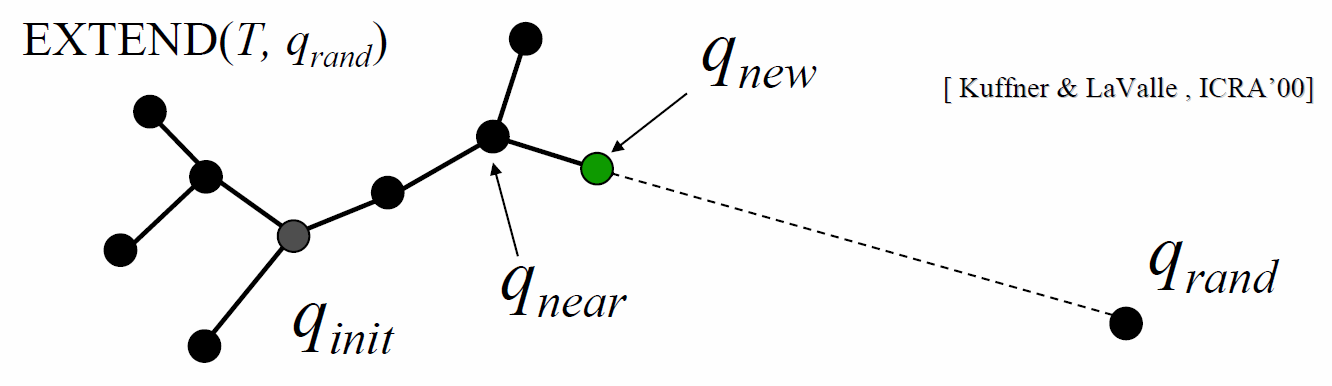
\includegraphics[width=.9\linewidth]{figure/rrt_extend}
		%\caption{}
		\label{fig:rrt_extend}
	\end{figure}
\end{frame}

\begin{frame}{RRT}{RRT$^{*}$}
	
\end{frame}


\begin{frame}{RRT$^{*}$}{RRT$^{*}$}
	
\end{frame}
